%% ============ SECTION 1 ============ %%
\section{Problem 1.}
\textit{
  Let $ z = f(x) = x^4 - 2x^2 - y^3 + 3y $.
  \begin{enumerate}[label=(\alph*)]
    \item Draw the graph of the function.
    \item Draw the contour plot of the function. Point out the local extreme
    and the saddle point on that figure.
    \item Find the exact local extreme and saddle point (using calculus
    technique).
  \end{enumerate}
}

\vspace*{1cm}

\textbf{Theory: }\\
We all know that the main uses of ordinary derivatives are to find maximum and minimum values (extreme values). Similar with multivariable functions, we can use partial derivatives to do the same thing.\\
Suppose we have a two-variable function $f$ that is continuous on the interval $(a,b)$ and it is said that:\\[6pt]
A function $f$ of two variables has a local maximum at $(a,b)$ if $f(x,y) \leq f(a,b)$ when $(x,y)$ is near $(a,b)$.
This means that $f(x,y) \leq f(a,b)$ for all points $(x,y)$ in some disk with center $(a,b)$. The number $f(a,b)$ is called a local maximum value. If $f(x,y) \geq f(a,b)$ when $(x,y)$ is near $(a,b)$, then $f$ has a local minimum at $(a,b)$ and $f(a,b)$ is a local minimum value.\\[6pt]
If the inequalities in the above definition hold for all points $(x,y)$ in the domain of $f$, then $f$ has an absolute maximum or local minimum at $(a,b)$.\\
Therefore, If $f$ has a local maximum or minimum at $(a,b)$ and the first-order partial derivatives of $f$ exist at that point, then $f_x(a,b) = 0$ and $f_y(a,b)=0$.\\[6pt]
But in some problems, There's a point called saddle point which located at the origin. Thus, we have another tool called \textbf{Second Derivatives Test} to determine which points are minimum, maximum and saddle.\\[6pt]
Assume that the second partial derivatives are continuous on a disk with center $(a,b)$, and suppose $f_x(a,b)=0$ and $f_y(a,b)=0$. Let:
$$ D(a,b) = f_{xx}(a,b) f_{yy}(a,b) - [f_{xy}(a,b)]^2 $$
If $D>0$ and $f_{xx}(a,b)>0$, then $f(a,b)$ is a local minimum.\\
If $D>0$ and $f_{xx}(a,b)<0$, then $f(a,b)$ is a local minimum.\\
If $D<0$, then $f(a,b)$ is not a local extrema, and the point $(a,b)$ is called a saddle point of $f$.\\
\textbf{Note}: If $D=0$, the test tells no information. $f$ could have a local maximum or local minimum at $(a,b)$, or $(a,b)$ could be a saddle point of $f$.\\

Finding the local extreme values of the function $f(x,y)$:
\begin{itemize}
  \item Identifying critical points for the given function $f(x,y)$.
    \begin{itemize}
      \item Find the partial derivatives with respect to $x$ and to $y$.
      \item Set each partial derivative equal to zero.
      \item Solve the system of equations to get critical points $(x_0,y_0)$.
    \end{itemize}

  \item Consider $D(x_0,y_0)$.
    \begin{itemize}
      \item Find all second derivatives of $f(x_0,y_0)$.
      \item Identify by the Second Derivative Test $ D(a,b) = f_{xx}(a,b) f_{yy}(a,b) - [f_{xy}(a,b)]^2 $
    \end{itemize}
\end{itemize}

\vspace*{1cm}

\textbf {MATLAB code: }
\begin{lstlisting}[style=Matlab-editor]
    %calculation
    syms x y z
    z = x.^2 + 2*y.^2 + 3*x.*y.^3 - y.^3;
    
    %differentiate z 
    fx = diff(z,x,1);   
    fy = diff(z,y,1);
    fxx = diff(z,x,2);
    fyy = diff(z,y,2);
    fxy = diff(fx,y,1);
    
    %create a system equation
    eqns = [ fx == 0, fy == 0];
    
    %define the variables for system equation
    vars = [x y];
    
    %solve the system equation
    [solx, soly] = vpasolve(eqns, vars);
    
    %only choose the real value
    solx_real = solx(imag(solx)==0);
    soly_real = soly(imag(solx)==0);
     
     
    %display section
    disp(['z = f(x,y) = ', char(z)])
    disp(['fx = ', char(fx)])
    disp(['fy = ', char(fy)])
    disp(['fxx = ', char(fxx)])
    disp(['fyy = ', char(fyy)])
    disp(['fxy = ', char(fxy)])
     
    %c
    for n=1:length(solx_real)
        fxx_val = subs(fxx,[x,y],[solx_real(n),soly_real(n)]);
    
    %calculate fxx, fyy, fxy values
    fyy_val = subs(fyy,[x,y],[solx_real(n),soly_real(n)]);
    fxy_val = subs(fxy,[x,y],[solx_real(n),soly_real(n)]);
    D = fxx_val*fyy_val - fxy_val*fxy_val;
    
    fprintf('\nFor point(%s,%s)\n',solx_real(n),soly_real(n))
        if D > 0
            fprintf('D = fxx*fyy-fxy^2 = %s\n',D)
            fprintf('So D > 0\n')
            fprintf('Therefore point (%s,%s) is local extreme\n',solx_real(n),soly_real(n))
            if fxx_val > 0
                fprintf('And fxx = %s\n',fxx_val)
                fprintf('So fxx > 0\n')
                fprintf('Therefore this is a local minimum point\n')
            else
                fprintf('And fxx = %s\n',fxx_val)
                fprintf('So fxx < 0\n')
                fprintf('Therefore this is a local maximum point\n')
            end
        elseif D < 0
            fprintf('D = fxx*fyy-fxy^2 = %s\n',D)
            fprintf('So D < 0\n')
            fprintf('Therefore point (%s,%s) is a saddle point\n',solx_real(n),soly_real(n))
        else
            fprintf('D = fxx*fyy-fxy^2 = %s\n',D)
            fprintf('So conclusion for point (%s,%s) \n',solx_real(n),soly_real(n))
        end
    end    
\end{lstlisting}

\begin{figure}[H]
  \centering
  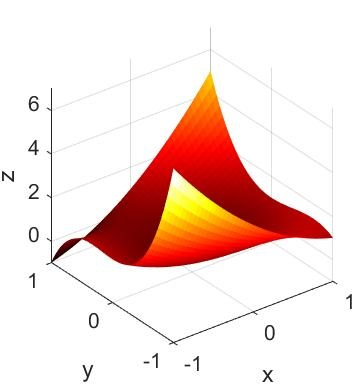
\includegraphics[width=12cm]{graphics/1a.jpg}
  \caption{The graph of the function $ z = f(x) = x^4 - 2x^2 - y^3 + 3y $.}
\end{figure}

\begin{lstlisting}[style=Matlab-editor]
    syms x y z
    [x,y] = meshgrid(-1:0.05:1,-1:0.05:1);
    z = x.^2 + 2*y.^2 + 3*x.*y.^3 - y.^3;

    %plot 2 figure in 1 window
    tiledlayout(2,1);

    %a
    nexttile
    surf(x,y,z,'edgecolor', 'none');
    colormap hot;   %the higher value, the hotter color
    xlabel('x');
    ylabel('y');
    zlabel('z');
    title('GRAPH OF THE FUNCTION')
    pbaspect([1,1,1])

    %b
    nexttile
    contour(x,y,z,200)
    hold on
    for n =1:length(solx_real)
        plot(solx_real(n),soly_real(n),'*')
    end
    xlabel('x');
    ylabel('y');
    title({'CONTOUR PLOT THE FUNCTION,','LOCAL EXTREME AND SADDLE POINT'})
    pbaspect([1,1,1])
\end{lstlisting}

\begin{figure}[H]
  \centering
  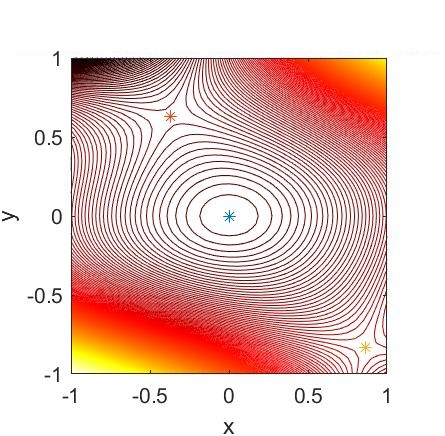
\includegraphics[width=12cm]{graphics/1b.jpg}
  \caption{The contour plot the function $ z = f(x) = x^4 - 2x^2 - y^3 + 3y $.}
\end{figure}

\vspace*{2cm}